%
% $Id: AttributeSet.java 15 2010-10-11 16:16:32Z justinkamerman $ 
%
% $LastChangedDate: 2010-10-11 13:16:32 -0300 (Mon, 11 Oct 2010) $ 
% 
% $LastChangedBy: justinkamerman $
%

\documentclass[10pt]{report}
\usepackage{graphicx}
\usepackage{setspace}			
\onehalfspacing

\title{CS6735 Programming Assignment 3}
\author{Justin Kamerman 3335272}
\date{\today}

\begin{document}
\maketitle
% No chapter numbers
\renewcommand*\thesection{\arabic{section}}

%----------------------------------------
% Assignment
%----------------------------------------
\section{Assignment}
\begin{enumerate} 
\item Read the following paper: 
\textit{Ron Kohavi, Scaling Up the Accuracy of Naive-Bayes Classifiers: a
Decision-Tree Hybrid. KDD-96.}
\\
You can download it from: 
http://robotics.stanford.edu/~ronnyk/ronnyk-bib.html
\item Implement the Na\"{\i}ve Bayes tree algorithm using Java. Evaluate
your implementation on the data sets in data.zip using 10 times 5-fold
cross-validation, and report the average accuracy and standard
deviation.  
\item Compare it with ID3 and Na\"{\i}ve Bayes in terms of accuracy. 

For breast cancer data see:
http://archive.ics.uci.edu/ml/datasets/Breast+Cancer+Wisconsin+%28Diagnostic%29

For car data see:
http://archive.ics.uci.edu/ml/datasets/Car+Evaluation

For ecoli data see:http://archive.ics.uci.edu/ml/datasets/Ecoli

For letter recognition data see:
http://archive.ics.uci.edu/ml/datasets/Letter+Recognition

For mushroom data see: http://archive.ics.uci.edu/ml/datasets/Mushroom

\item \textbf{Bonus question:} Change your implementation to output AUC, and
  compare NBtree with ID3 and Na\"{\i}ve Bayes in terms of AUC. 
\end{enumerate}

%----------------------------------------
% Learning Algorithm
%----------------------------------------
\section{Learning Algorithm}
\label{sec:learningalgorithm}
The program implements the NBTree algorithm
described in \cite{RefWorks:63}. While the NBTree algorithm is
recursive, it has been implemented iteratively using an application
stack. This is a personal preference of the student based on past
experience with recursive programming causing JVM stack overflow
problems.

In the NBTree implementation, a Na\"{\i}ve Bayes classifier is created
at every tree node, not just leaf nodes. Non-leaf Na\"{\i}ve Bayes
classifiers are used during classification when there is no edge
leaving a node corresponding to the attribute value being
examined. This is analogous to storing a default classification at
each non-leaf node in the Decision Tree implementation of assignment 1
to allow classification of instances for which no path was constructed
to a leaf during training.

Missing attribute values are handled by preprocessing data sets,
replacing missing attribute value with the most probable value for the
attribute in the data set.


%----------------------------------------
% Data Sets
%----------------------------------------
\section{Data Sets}
Program expects data in CSV format with attributes occurring first and
classification at the end of each line. All data files have been
preprocessed to fit this format.


\subsection*{car.data}
\begin{itemize}
\item Number of Instances: 1728
\item Number of Attributes: 6
\item Attribute Values:
  \\\\
  \begin{left}
    \begin{tabular}{ l l }
      buying     & v-high, high, med, low \\
      maint      & v-high, high, med, low \\
      doors      & 2, 3, 4, 5-more \\
      persons    & 2, 4, more \\
      lug\_boot  & small, med, big \\
      safety     & low, med, high \\
    \end{tabular}
  \end{left}
  \\
\item Missing Attribute Values: none
\item Class Distribution (number of instances per class)
  \\\\
  \begin{left}
    \begin{tabular}{ l l }
      unacc   &  1210 \\
      acc     &   384 \\   
      good    &    69 \\     
      v-good  &    65 \\
    \end{tabular}
  \end{left}
\end{itemize}


\subsection*{ecoli.data}
\begin{itemize}
\item Number of Instances:  336
\item Number of Attributes: 7 
\item Attribute Values:
  \\\\
  \begin{left}
    \begin{tabular}{ l p{10cm} }
      mcg  &   McGeoch's method for signal sequence recognition. \\
      gvh  &   von Heijne's method for signal sequence recognition. \\
      lip  &   von Heijne's Signal Peptidase II consensus sequence score. Binary attribute. \\
      chg  &   Presence of charge on N-terminus of predicted lipoproteins. Binary attribute. \\
      aac  &   score of discriminant analysis of the amino acid content of outer membrane and periplasmic proteins. \\
      alm1 &   score of the ALOM membrane spanning region prediction program. \\
      alm2 &   score of ALOM program after excluding putative cleavable signal regions from the sequence. \\
    \end{tabular}
  \end{left}
  \\   
\item Missing Attribute Values: none.
\item Class Distribution (number of instances per class)
  \\\\
  \begin{left}
    \begin{tabular}{ l l }
      cp    &      143 \\
      im    &       77 \\               
      pp    &       52 \\
      imU   &       35 \\
      om    &       20 \\
      omL   &        5 \\
      imL   &        2 \\
      imS   &        2 \\
    \end{tabular}
  \end{left}
\end{itemize}


\subsection*{mushroom.data}
\begin{itemize}
\item Number of Instances: 8124
\item Number of Attributes: 22
\item Attribute Information:
  \\\\
  \begin{left}
    \begin{tabular}{ l p{10cm} }
      cap-shape                 &     bell=b, conical=c, convex=x, flat=f, knobbed=k, sunken=s \\
      cap-surface               &     fibrous=f, grooves=g, scaly=y, smooth=s \\
      cap-color                 &     brown=n, buff=b, cinnamon=c, gray=g, green=r, pink=p, purple=u, red=e, white=w, yellow=y \\
      bruises?                  &     bruises=t, no=f \\
      odor                      &     almond=a, anise=l, creosote=c, fishy=y, foul=f, musty=m, none=n, pungent=p, spicy=s \\
      gill-attachment           &     attached=a, descending=d, free=f, notched=n \\
      gill-spacing              &     close=c, crowded=w, distant=d \\
      gill-size                 &     broad=b, narrow=n \\
      gill-color                &     black=k, brown=n, buff=b, chocolate=h, gray=g, green=r, orange=o, pink=p, purple=u, red=e, white=w, yellow=y \\
      stalk-shape               &     enlarging=e, tapering=t \\
      stalk-root                &     bulbous=b, club=c, cup=u, equal=e, rhizomorphs=z, rooted=r, missing=? \\
      stalk-surface-above-ring  &     fibrous=f, scaly=y, silky=k, smooth=s \\
      stalk-surface-below-ring  &     fibrous=f, scaly=y, silky=k, smooth=s \\
      stalk-color-above-ring    &     brown=n, buff=b, cinnamon=c, gray=g, orange=o, pink=p, red=e, white=w, yellow=y \\
      stalk-color-below-ring    &     brown=n, buff=b, cinnamon=c, gray=g, orange=o, pink=p, red=e, white=w, yellow=y \\
      veil-type                 &     partial=p, universal=u \\
      veil-color                &     brown=n, orange=o, white=w, yellow=y \\
      ring-number               &     none=n, one=o, two=t \\
      ring-type                 &     cobwebby=c, evanescent=e, flaring=f, large=l, none=n, pendant=p, sheathing=s, zone=z \\
      spore-print-color         &     black=k, brown=n, buff=b, chocolate=h, green=r, orange=o, purple=u, white=w, yellow=y \\
      population                &     abundant=a, clustered=c, numerous=n, scattered=s, several=v, solitary=y \\
      habitat                   &     grasses=g, leaves=l, meadows=m, paths=p, urban=u, waste=w, woods=d \\
    \end{tabular}
  \end{left}

\item Missing Attribute Values: 2480, all for attribute #11.
\item Class Distribution: 
  \\\\
  \begin{left}
    \begin{tabular}{ l l }
      edible:     &  4208 (51.8\%) \\
      poisonous:  &  3916 (48.2\%) \\
      total:      &  8124 instances \\
    \end{tabular}
  \end{left}
\end{itemize}


\subsection*{letter-recognition.data}
\begin{itemize}
\item Number of Instances: 20000
\item Number of Attributes: 17 (Letter category and 16 numeric features)
\item Attribute Information:
  \\\\
  \begin{left}
    \begin{tabular}{ l p{10cm} }
      lettr	   &    capital letter	(26 values from A to Z) \\
      x-box	   &    horizontal position of box	(integer) \\
      y-box	   &    vertical position of box	(integer) \\
      width	   &    width of box			(integer) \\
      high 	   &    height of box			(integer) \\
      onpix	   &    total # on pixels		(integer) \\
      x-bar	   &    mean x of on pixels in box	(integer) \\
      y-bar	   &    mean y of on pixels in box	(integer) \\
      x2bar	   &    mean x variance			(integer) \\
      y2bar	   &    mean y variance			(integer) \\
      xybar	   &    mean x y correlation		(integer) \\
      x2ybr	   &    mean of x * x * y		(integer) \\
      xy2br	   &    mean of x * y * y		(integer) \\
      x-ege	   &    mean edge count left to right	(integer) \\
      xegvy	   &    correlation of x-ege with y	(integer) \\
      y-ege	   &    mean edge count bottom to top	(integer) \\
      yegvx	   &    correlation of y-ege with x	(integer) \\
    \end{tabular}
  \end{left}

\item Missing Attribute Values: None
\item Class Distribution:
  \\\\
  \begin{left}
    \begin{tabular}{ l l l l l l l }
 	789 A	   & 766 B     & 736 C     & 805 D	 & 768 E	   & 775 F     & 773 G \\
 	734 H	   & 755 I     & 747 J     & 739 K	 & 761 L	   & 792 M     & 783 N \\
 	753 O	   & 803 P     & 783 Q     & 758 R	 & 748 S	   & 796 T     & 813 U \\
 	764 V	   & 752 W     & 787 X     & 786 Y	 & 734 Z \\
    \end{tabular}
  \end{left}
\end{itemize}


\subsection*{breast-cancer.data}
\begin{itemize}
\item Number of Instances: 699
\item Number of Attributes: 10
\item Attribute Information: (class attribute has been moved to last column)
  \\\\
  \begin{left}
    \begin{tabular}{ l l }
      Clump Thickness               &  1 - 10  \\
      Uniformity of Cell Size       &  1 - 10  \\
      Uniformity of Cell Shape      &  1 - 10  \\
      Marginal Adhesion             &  1 - 10  \\
      Single Epithelial Cell Size   &  1 - 10  \\
      Bare Nuclei                   &  1 - 10  \\
      Bland Chromatin               &  1 - 10  \\
      Normal Nucleoli               &  1 - 10  \\
      Mitoses                       &  1 - 10  \\
    \end{tabular}
  \end{left}

\item Missing attribute values: 16
\item Class distribution: (2 for benign, 4 for malignant)
  \\\\
  \begin{left}
    \begin{tabular}{ l l }
      Benign       &  458 (65.5\%) \\
      Malignant    &  241 (34.5\%) \\
    \end{tabular}
  \end{left}
\end{itemize}


%----------------------------------------
% Program Design
%----------------------------------------
\section{Program Design}
The NBTree \cite{RefWorks:63} algorithm is implemented by a Java
program. The only external dependency is on the Apache commons-cli
library for parsing commend line options. To that end, the program is
operated from the command line, taking options listed in table
\ref{tab:commandline}.  

\begin{table}[h]
  \centering
  \begin{tabular}{ |l|p{10cm}|} 
    \hline
    Option & Description \\ \hline
    -d          &  Generate Graphviz DOT output. \\ \hline
    -f \<arg\>  &  Path of data file \\ \hline
    -i \<arg\>  &  Number of iterations to perform. Default is 10 \\ \hline
    -n \<arg\>  &  A comma-separated list of attribute names, matching
    the order in which they appear in the data file \\ \hline
    -o \<arg\>  &  Number of folds to create in the training data during. Default is 5. \\ \hline
    -h          &  Print help message \\ \hline
  \end{tabular}
  \caption{Command line options}
  \label{tab:commandline}
\end{table}

The program parses a data file, assumed to contain a set of training
instances on each line. Each training instance line is a
comma-separated list of attribute values terminated by a
classification or target value. Of the training data supplied for the
assignment, some had to be preprocessed to fit the expected format.

The program then executes a number of iterations (default is 10) over
the entire data set. During each iteration, the data set is folded
(default is 5 times), the training set used to create an NBTree. The
instances in the test set are then evaluated by the NBTree. The
accuracy of the classifications is recorded 
for each test set evaluated. After the final iteration is complete,
the mean accuracy and standard deviation are calculated and output by
the program.

The program implements various mechanism to facilitate
debugging. Throughout the code, log statements have been added using
the Java logging framework. The logging output is controlled for
individual classes via the \textit{logging.properties} file which the program
read on startup. In addition to logging, code was added to generate
Graphviz DOT \cite{Graphviz2001} output representing
the NBTree created. This output can be rendered using Graphviz
dot tool. 

\begin{figure}
  \begin{center}
	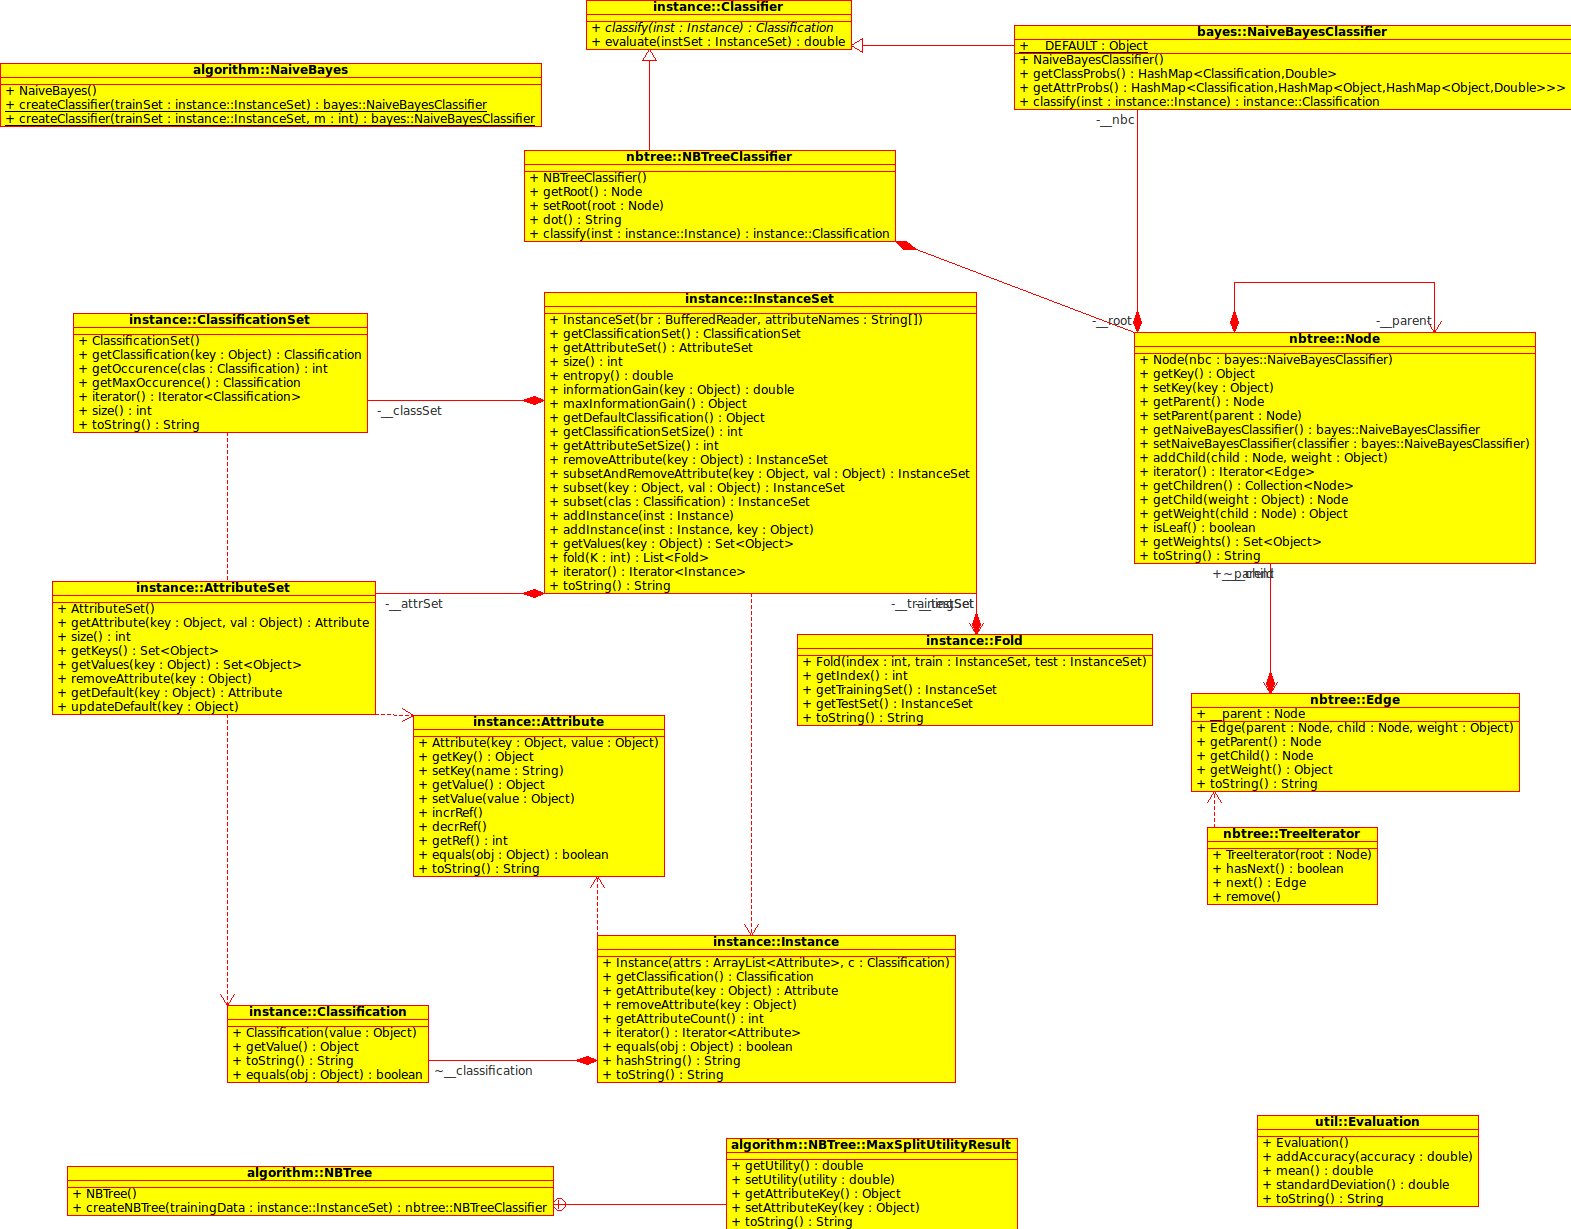
\includegraphics[angle=90,width=\textwidth,height=!]{uml}
  \end{center}
  \caption{UML class diagram}
  \label{fig:uml}
\end{figure} 

The implementation classes and their relationships are represented in a UML
class diagram in Figure \ref{fig:uml}. Following is a brief
description of each class:

\begin{itemize}
\item \textbf{Attribute} represents an attribute's name and value.

\item \textbf{AttributeSet} is a collection of attributes. It has
  convenience functions to determine attribute value range and
  probabilities of discrete values.

\item \textbf{Classification} represents an instance's classification
  or the value of the target function.

\item \textbf{ClassificationSet} is a collection of
  classifications. It has convenience functions to determine
  classification value range and probabilities of each
  classification. These functions are used extensively during the
  entropy calculation. 

\item \textbf{Classifier} is an interface implemented by any class
  which can take an instance and generate a classification for that
  instance. The interface is implemented by the \textit{NBTree} and
  \textit{NaiveBayesClassifier}.


\item \textbf{Edge} represents an edge in an \textit{NBTree}. Each Edge
  is associated with an attribute value.

\item \textbf{Evaluation} is a helper class for capturing test run
  accuracies and calculating final mean and standard deviation values.

\item \textbf{Fold} is an encapsulation of a training and a test set.

\item \textbf{Instance} represents a collection of attributes and
  their classification. In the case of training data, we use the
  classification to select the target hypothesis. In the case of test
  data, the classification is used to validate output of the target
  hypothesis.

\item \textbf{InstanceSet} is a collection of \textit{Instances}. This is the
  class that parses the data file and generates individual
  Instances. Functions exist to calculate entropy and information
  gain, create a subset of instance based on a particular attribute's
  value and fold the set of instances to create test and training sets
  of instances.

\item \textbf{LogFormatter} is a helper class to format log messages.

\item \textbf{NBTreeMain} is the class which is started from the command
  line. It parses command line options and starts the test iterations.

\item \textbf{NaiveBayes} creates a Na\"{\i}ve Bayes Classifier
  given a training data \textit{InstanceSet}. It calculates marginal
  and conditional probabilities and populates a probability matrix
  within the \textit{NaiveBayesClassifier}. It uses the m-estimation
  technique to estimate conditional probabilities.

\item \textbf{NaiveBayesClassifier} classifies an \textit{Instance}
  using the Na\"{i}ve Bayes Classifier, based on a matrix of
  marginal and conditional probabilities which are calculated from a
  previously seen training set.

\item \textbf{NBTree} creates an \textit{NBTreeClassifier} given a
  training data \textit{InstanceSet}.

\item \textbf{NBTreeClassifier} classifies an \textit{Instance}
  using the encapsulated tree structure and associated
  \textit{NaiveBayesClassifier} instances created during training.

\item \textbf{Node} represents a node in an \textit{NBTree}. Each node is
  associated with either a particular attribute or classification
  depending on whether the node is an internal or leaf
  respectively. 

\item \textbf{TreeIterator} is a helper class for performing a
  depth-first traversal of the \textit{NBTree}.

\end{itemize}


%----------------------------------------
% Results
%----------------------------------------
\section{Results}
\label{sec:results}
The results of processing each data file using the NBTree
implementation are summarized in Table 
\ref{tab:comparison}. In general, learning time was significantly
higher than both the ID3 and Na\"{i}ve Bayes learning
algorithms. Intuitively, this was expected because of the large number
of Na\"{i}ve Bayes classifiers that are created and evaluated during
the utility calculation.

All tests were run on a personal computer with an AMD Athlon 64 2GHz
Processor, 1GB RAM, running a 32 bit Linux 2.6.31 kernel. The Java
Virtual Machine used was version 1.6.0-18.
\\
\begin{table}[h]
  \centering
  \begin{tabular}{ |l|r|r|r|r|} 
    \hline
    \textbf{Data Set} & \textbf{Na\"{i}ve Bayes} & \textbf{ID3} & \textbf{NBTree 5\%} & \textbf{NBTree 3\%} \\ \hline
    car                      &  0.841449  &  0.938377  & 0.882783  & 0.925797 \\ \hline
    ecoli                    &  0.684776  &  0.384776  & 0.674328  & 0.668657 \\ \hline
    mushroom                 &  0.952007  &  1.000000  & 0.951850  & 0.996921 \\ \hline
    letter-recognition       &  0.737670  &  0.760870  & 0.819500  &          \\ \hline
    breast-cancer-wisconsin  &  0.972662  &  0.945899  & 0.972806  & 0.971223 \\ \hline
  \end{tabular}
  \caption{Comparison of Na\"{i}ve Bayes, ID3, and
    NBTree accuracy over benchmark data sets. NBTree results for both
    3\% and 5\% split utility thresholds are shown}
  \label{tab:comparison}
\end{table}


\subsection*{car.data}
Using a split utility threshold of 5\%, the car evaluation was run
through 10 iterations of 5-fold cross-validation. Calculated
\textbf{mean accuracy} was 0.882783 and 
\textbf{standard deviation} 0.047129. The NBTree split utility
threshold of 5\% relative improvement in accuracy, did not justify a
split on any attribute. Essentially, this is a Na\"{i}ve Bayes
classifier and evaluation results are within a single standard
deviation of the results of the previous assignment.

The data set was re-evaluated using a split utility threshold of 3\%,
resulting in improved \textbf{mean accuracy} of 0.925797 and 
\textbf{standard deviation} 0.01811. The lower split threshold drove
the formation of the NBTree structure shown in Figure \ref{fig:car}.

\begin{figure}
  \begin{center}
	
\includegraphics[width=\textwidth,height=!]{car}
  \end{center}
  \caption{NBTree visualization generated for car data set with 3\%
    split utility threshold}
  \label{fig:car}
\end{figure} 

\subsection*{ecoli.data}
Using a split utility threshold of 5\%, the ecoli evaluation was run
through 10 iterations of 5-fold 
cross-validation. Calculated \textbf{mean accuracy} was 0.674328 and 
\textbf{standard deviation} 0.057782. Although the NBTree split utility
threshold of 5\% relative improvement in accuracy, justified a split,
the resulting tree did not perform significantly better than the
Na\"{i}ve Bayes classifier in the previous assignment. The NBTree
structure produced for one of cross-validation folds is shown in Figure
\ref{fig:ecoli}. 

The data set was re-evaluated using a split utility threshold of 3\%. The
adjusted threshold did not see a significant change in accuracy,
yielding \textbf{mean accuracy} of 0.668657 and \textbf{standard
  deviation} 0.061466.

\begin{figure}
  \begin{center}
	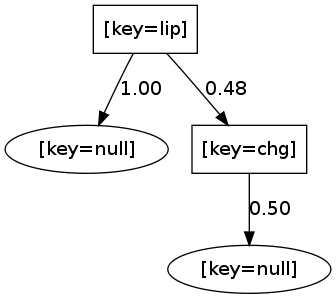
\includegraphics[width=0.5\textwidth,height=!]{ecoli}
  \end{center}
  \caption{NBTree visualization generated for ecoli data set with 5\%
    utility }
  \label{fig:ecoli}
\end{figure} 


\subsection*{mushroom.data}
Using a split utility threshold of 5\%, the mushroom evaluation was
run through a single iteration of 5-fold
cross-validation. The full 10 iterations required was not completed
due to time constraints, a single fold taking in excess of three hours
to complete. Calculated \textbf{mean accuracy} was 0.95185 and
\textbf{standard deviation} 0.00856. The NBTree split utility
threshold of 5\% relative improvement in accuracy, did not justify a
split on any attribute. Essentially, this is a Na\"{i}ve Bayes
classifier and evaluation results are within a single standard
deviation of the results of the previous assignment.

The data set was re-evaluated using a split utility threshold of 3\%,
yielding an \textbf{accuracy} of 0.996921. Time
constraints only permitted evaluation of a single fold so it it is
impossible to assess the accuracy variance. The lower split threshold drove
the formation of the NBTree structure shown in Figure \ref{fig:mushroom}.

\begin{figure}
  \begin{center}
	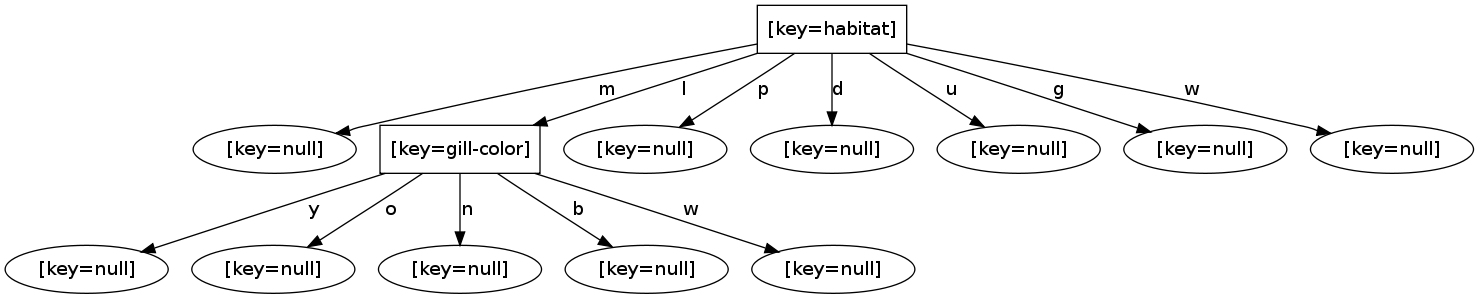
\includegraphics[width=\textwidth,height=!]{mushroom}
  \end{center}
  \caption{NBTree visualization generated for mushroom data set with 3\%
    utility }
  \label{fig:mushroom}
\end{figure} 

\subsection*{letter-recognition.data}
The letter-recognition evaluation ran a single fold of 5-fold
cross-validation. The full 10 iterations of 5-fold cross validation
required was not completed due to time constraints, a single fold
taking in excess of twelve hours to complete. \textbf{Accuracy} for
the single fold was 0.819500. It is difficult to say so with
conviction given the sparse evaluation results, but this data set
seems to be the only one tested to show a possible improvement over
ID3 or Na\"{i}ve Bayes. Perhaps it is not co-incidental that this data
set resulted in the largest tree structure. The tree produced for one
of the cross-validation folds is shown in Figure
\ref{fig:letter-recognition}. 

Due to time constraints no attempt was made to investigate the effects
of adjusting the split utility threshold.

\begin{figure}
  \begin{center}
	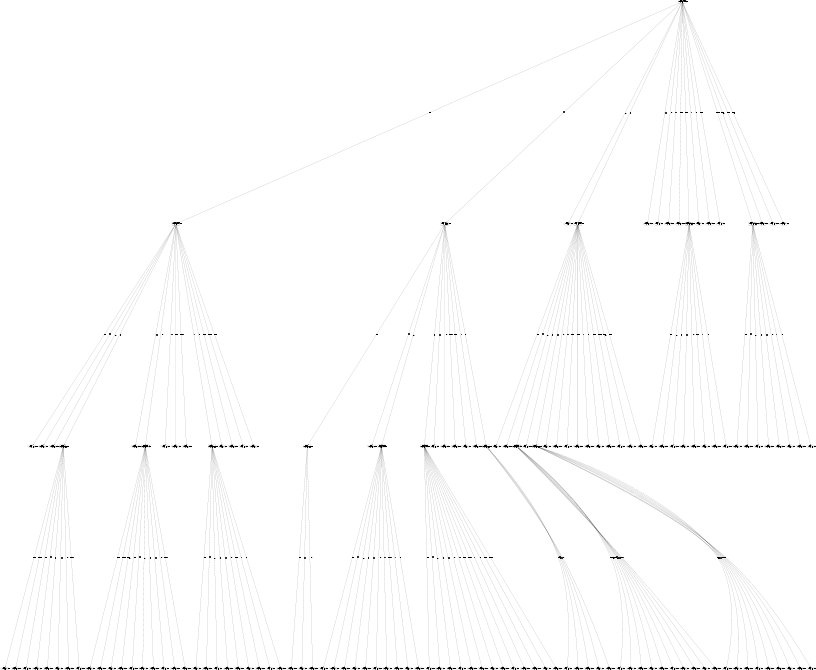
\includegraphics[angle=90,width=!,height=\textheight]{letter-recognition}
  \end{center}
  \caption{NBTree visualization generated for letter-recognition data
    set with 5\% split utility threshold}
  \label{fig:letter-recognition}
\end{figure} 


\subsection*{breast-cancer.data}
The breast-cancer evaluation ran 10 iterations of 5-fold cross
validation. Calculated \textbf{mean accuracy} was 0.972806 and
\textbf{standard deviation} 0.012568. The NBTree split utility
threshold of 5\% relative improvement in accuracy, did not justify a
split on any attribute. Essentially, this is a Na\"{i}ve Bayes
classifier and evaluation results are within a single standard
deviation of the results of the previous assignment.

The data set was re-evaluated using split utility thresholds of 3\%,
2\%, and 1\%. However none of these thresholds produced a split in the
NBTree.


%----------------------------------------
% Bibliography
%----------------------------------------
\bibliography{bibliography}
\bibliographystyle{plain}


%--------------------------------------------------
\end{document}
